\section{Full cited-pair census and run-stability sensitivity}
\label{app:scifact3-census}
The post-hoc census includes all 339 eligible SciFact development claim--explicitly-cited-abstract pairs: 138 SUPPORT, 71 CONTRADICT and 130 derived \textsc{NoInfo}. Its 159-pair complement to the earlier balanced three-choice selection contains 78/11/70 by class. This complement is not a held-out source: selected and complement pairs share 21 claims and 41 documents, and 37 complement positives appeared in our earlier two-choice task. Every one of the five systems received all four freshly generated conditions on all 339 pairs (1,356 requests/system). The freeze was fixed before this fresh inference, but the census question followed inspection of the selected-180 results. All base/reversal outputs were valid; Jev had one invalid decision under title removal only.

\begin{table}[h]
\centering\small\setlength{\tabcolsep}{4pt}
\begin{tabular}{lrrrr}
\toprule
System & Full 339 B$\to$R & Complement 159 B$\to$R & Comp. \textsc{NoInfo} 70 & Flip / repeat \\
\midrule
Laya English & 171$\to$164 & 90$\to$88 & 16$\to$13 & 29 / 0 \\
Laya Multilingual & 150$\to$150 & 77$\to$80 & 8$\to$8 & 63 / 0 \\
Llama 3.1 8B & 182$\to$158 & 103$\to$90 & 33$\to$15 & 73 / 0 \\
Qwen3 8B & 231$\to$220 & 129$\to$119 & 60$\to$38 & 97 / 0 \\
Jev 1.13 & 291$\to$292 & 144$\to$143 & 59$\to$59 & 5 / 4 \\
\bottomrule
\end{tabular}
\caption{Fresh-run reference-correct counts and valid semantic base-to-reversal/repeat flips. The option reversal is a joint display-plus-answer-code change for code-likelihood adapters. The complement is within the same source, not an independent data set.}
\end{table}

For Qwen on the complement, the paired claim-cluster 95\% interval for the \textsc{NoInfo} accuracy difference is $[-42.4,-21.1]$ percentage points; document-cluster sensitivity gives $[-42.9,-20.3]$. The overall difference is $-6.3$ points with claim interval $[-13.7,+1.2]$. These are fixed-development-source, pointwise descriptive intervals, not uncertainty over scientific domains or reference validity. The 11 complement contradictions span only six claim clusters; their apparent $4\to7$ improvement is especially imprecise. \textsc{NoInfo} remains an explicitly cited pair with no annotated abstract-evidence entry, not an independently adjudicated neutral relation.

An overlap audit matched all 720 earlier selected-180 request hashes to the fresh census and every available tokenized-prompt hash for both local LLMs. Nevertheless, two Qwen selected-180 base \textsc{NoInfo} predictions changed to SUPPORT across runs, yielding prior $104/180$ versus fresh $102/180$ base correctness; reversal stays $101/180$. The batch size stayed four, but co-batches differed, and the audit does not identify the cause. The fresh census is therefore never assembled by combining prior and complement outputs. An offline common-semantic tie-break changes full-census reversed correct counts only from $158\to159$ for Llama and $220\to219$ for Qwen. Raw hashes, case-level transitions, cluster resampling and reference-provenance sidecars are retained in \texttt{research/scifact3\_census\_v1/}; access and upstream-license review are pending.

\raggedbottom
\subsection{Execution-context stability is not interface invariance}
\label{sec:batch-context}
Motivated by the cross-run drift above, we froze a new follow-up before its own inference: all 339 census pairs in both base and joint-reversal conditions, two local LLMs, and five execution plans (6,780 decisions). The plans are original contiguous batches of four, an identical repeat in the same process, reversal of row order within the same batches, seeded reassignment to new batches of four, and single-request execution. No case is selected by its reference, prior error or logit margin. The unchanged adapter uses the pinned weights, chat template, BF16/SDPA and explicit position IDs; every unpadded prompt-token and request hash matches across plans and against the prior census. Only execution context changes, not the model-facing candidate interface.

Both models have zero semantic flips under identical-batch repeat and within-batch row reversal. Repacking changes 1 base and 4 reversed-condition Qwen predictions, versus 3 and 5 for Llama. Singleton execution changes 3 and 3 Qwen predictions, versus 7 and 5 for Llama, respectively; each count has denominator 339 (Figure~\ref{fig:batch-context}). Original top-two candidate-logit margins of these changed decisions are at most 0.5 for Qwen and 0.375 for Llama; several are exact BF16 ties. Native tie decoding is retained. The original-plan semantic labels reproduce the previous full census for both models. Nonetheless, across all five plans, joint option reversal still changes 95--97 Qwen and 71--73 Llama predictions. The derived \textsc{NoInfo} reference-agreement difference stays between $-34.6$ and $-33.1$ percentage points for Qwen and between $-27.7$ and $-26.9$ for Llama. Each plan's paired claim-cluster 95\% interval excludes zero; these are pointwise descriptive intervals on the fixed source, not independent replications across plans.

\begin{figure}[H]
\centering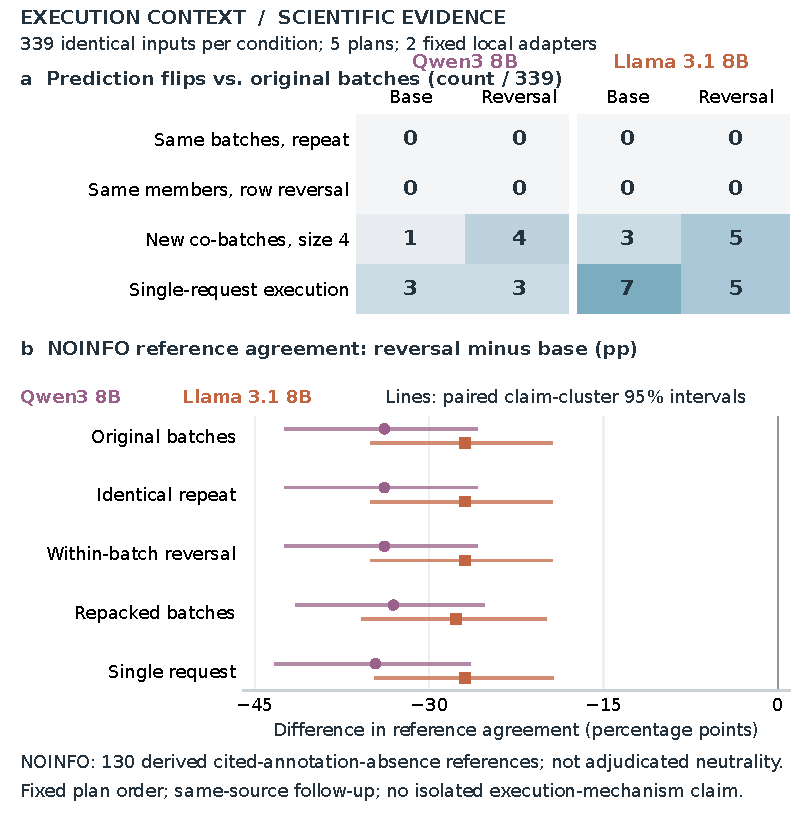
\includegraphics[width=.99\linewidth]{figures/fig_batch_context.pdf}
\caption{Execution-context follow-up on all 339 SciFact cited pairs. (a) Same-condition semantic flips relative to original contiguous batches; columns distinguish base and joint option reversal. (b) Reversal-minus-base reference agreement on all 130 derived \textsc{NoInfo} pairs, with 10,000-draw paired claim-cluster percentile intervals. Execution perturbations move few predictions while the class-specific interface effect persists. \textsc{NoInfo} is cited annotation absence, not adjudicated neutrality. Fixed execution-plan order is not counterbalanced.}
\label{fig:batch-context}
\end{figure}

This control supports robustness of the class-level interface pattern to the tested execution contexts, not bitwise determinism or a unique numerical mechanism. Repacking and singleton execution also change padding and kernel shapes; the fixed plan order does not isolate time-dependent effects. Same-process repeats do not establish cross-process, cross-GPU or cross-version reproducibility. These new outputs remain separate from historical results in \texttt{research/batch\_context\_v1/}.

\paragraph{Reference audit prepared, not completed.} A source-verified blinded work package includes all 130 derived \textsc{NoInfo} pairs plus 15 annotated support and 15 contradiction calibration pairs. Two independently randomized packets omit reference labels, strata and model outputs; independent annotation forms are blank. The workflow retains four-way agreement (including UNCERTAIN), separate derived/calibration statistics, locked form hashes and third-reviewer adjudication. Source-containing packets remain restricted and precisely ignored by version control. No human-validity result is claimed until independent reviewers complete this work.

